% Owner: Samriddhi (Member 4)
\subsection{Phase II timing behaviour}
Fig.~\ref{fig:wave2} is generated from the VCD of \sig{memcopy} on the modified Harvard system
with $L=4$. In cycles 8--11 the I-cache misses on PC \texttt{0x010}: \sig{i\_ready} is low, the
arbiter grants the instruction side, and \sig{m\_ready} rises in the fourth cycle. The LW then
misses in the D-cache (cycles 12--15, physical \texttt{0x400}) and completes as a hit in cycle
16. The SW in cycle 17 finds the write buffer empty and is offered to memory. Memory does not
finish it in that cycle, so the buffer captures it, \sig{d\_ready} stays high and the core goes
on to execute \texttt{0x018} and \texttt{0x01c} while the store drains (\sig{wb\_busy}). In cycle
20 the next instruction misses while the D-side still owns the memory. This is a conflict cycle:
because there is no pre-emption, the instruction refill starts only in cycle 21.

\begin{figure*}[t]
  \centering
  \resizebox{\textwidth}{!}{% generated by tools/vcd2tikz.py from tb_system_memcopy.vcd -- do not edit
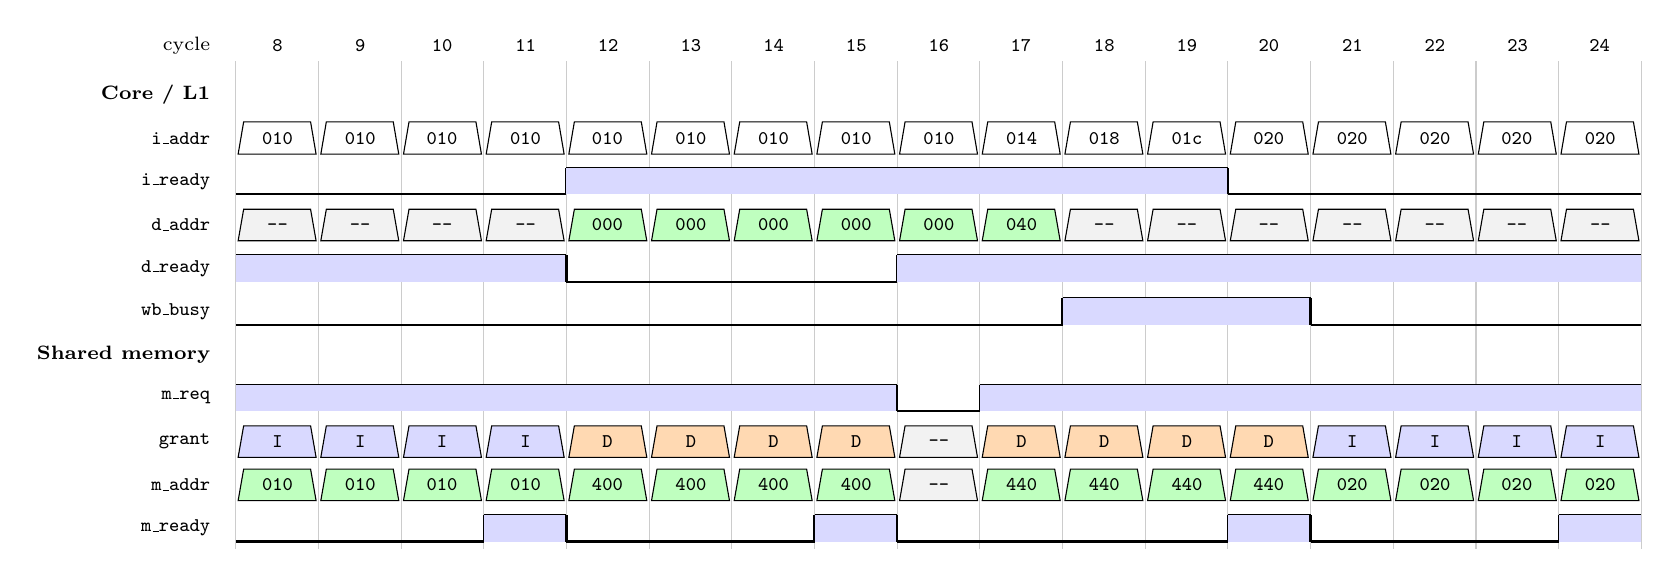
\begin{tikzpicture}[font=\scriptsize\ttfamily, x=1cm, y=1cm]
\node at (0.53,0.35) {8};
\node at (1.58,0.35) {9};
\node at (2.62,0.35) {10};
\node at (3.68,0.35) {11};
\node at (4.73,0.35) {12};
\node at (5.78,0.35) {13};
\node at (6.83,0.35) {14};
\node at (7.88,0.35) {15};
\node at (8.93,0.35) {16};
\node at (9.97,0.35) {17};
\node at (11.03,0.35) {18};
\node at (12.08,0.35) {19};
\node at (13.12,0.35) {20};
\node at (14.18,0.35) {21};
\node at (15.23,0.35) {22};
\node at (16.28,0.35) {23};
\node at (17.32,0.35) {24};
\node[anchor=east] at (-0.2,0.35) {\normalfont cycle};
\draw[gray!40] (0.00,0.15) -- (0.00,-6.05);
\draw[gray!40] (1.05,0.15) -- (1.05,-6.05);
\draw[gray!40] (2.10,0.15) -- (2.10,-6.05);
\draw[gray!40] (3.15,0.15) -- (3.15,-6.05);
\draw[gray!40] (4.20,0.15) -- (4.20,-6.05);
\draw[gray!40] (5.25,0.15) -- (5.25,-6.05);
\draw[gray!40] (6.30,0.15) -- (6.30,-6.05);
\draw[gray!40] (7.35,0.15) -- (7.35,-6.05);
\draw[gray!40] (8.40,0.15) -- (8.40,-6.05);
\draw[gray!40] (9.45,0.15) -- (9.45,-6.05);
\draw[gray!40] (10.50,0.15) -- (10.50,-6.05);
\draw[gray!40] (11.55,0.15) -- (11.55,-6.05);
\draw[gray!40] (12.60,0.15) -- (12.60,-6.05);
\draw[gray!40] (13.65,0.15) -- (13.65,-6.05);
\draw[gray!40] (14.70,0.15) -- (14.70,-6.05);
\draw[gray!40] (15.75,0.15) -- (15.75,-6.05);
\draw[gray!40] (16.80,0.15) -- (16.80,-6.05);
\draw[gray!40] (17.85,0.15) -- (17.85,-6.05);
\node[anchor=east,font=\normalfont\bfseries\scriptsize] at (-0.2,-0.28) {Core / L1};
\node[anchor=east] at (-0.2,-0.83) {i\_addr};
\draw[fill=white] (0.03,-1.03) -- (0.10,-0.62) -- (0.95,-0.62) -- (1.02,-1.03) -- cycle;
\node at (0.53,-0.83) {010};
\draw[fill=white] (1.08,-1.03) -- (1.15,-0.62) -- (2.00,-0.62) -- (2.07,-1.03) -- cycle;
\node at (1.58,-0.83) {010};
\draw[fill=white] (2.13,-1.03) -- (2.20,-0.62) -- (3.05,-0.62) -- (3.12,-1.03) -- cycle;
\node at (2.62,-0.83) {010};
\draw[fill=white] (3.18,-1.03) -- (3.25,-0.62) -- (4.10,-0.62) -- (4.17,-1.03) -- cycle;
\node at (3.68,-0.83) {010};
\draw[fill=white] (4.23,-1.03) -- (4.30,-0.62) -- (5.15,-0.62) -- (5.22,-1.03) -- cycle;
\node at (4.72,-0.83) {010};
\draw[fill=white] (5.28,-1.03) -- (5.35,-0.62) -- (6.20,-0.62) -- (6.27,-1.03) -- cycle;
\node at (5.78,-0.83) {010};
\draw[fill=white] (6.33,-1.03) -- (6.40,-0.62) -- (7.25,-0.62) -- (7.32,-1.03) -- cycle;
\node at (6.83,-0.83) {010};
\draw[fill=white] (7.38,-1.03) -- (7.45,-0.62) -- (8.30,-0.62) -- (8.37,-1.03) -- cycle;
\node at (7.88,-0.83) {010};
\draw[fill=white] (8.43,-1.03) -- (8.50,-0.62) -- (9.35,-0.62) -- (9.42,-1.03) -- cycle;
\node at (8.93,-0.83) {010};
\draw[fill=white] (9.48,-1.03) -- (9.55,-0.62) -- (10.40,-0.62) -- (10.47,-1.03) -- cycle;
\node at (9.98,-0.83) {014};
\draw[fill=white] (10.53,-1.03) -- (10.60,-0.62) -- (11.45,-0.62) -- (11.52,-1.03) -- cycle;
\node at (11.03,-0.83) {018};
\draw[fill=white] (11.58,-1.03) -- (11.65,-0.62) -- (12.50,-0.62) -- (12.57,-1.03) -- cycle;
\node at (12.08,-0.83) {01c};
\draw[fill=white] (12.63,-1.03) -- (12.70,-0.62) -- (13.55,-0.62) -- (13.62,-1.03) -- cycle;
\node at (13.12,-0.83) {020};
\draw[fill=white] (13.68,-1.03) -- (13.75,-0.62) -- (14.60,-0.62) -- (14.67,-1.03) -- cycle;
\node at (14.18,-0.83) {020};
\draw[fill=white] (14.73,-1.03) -- (14.80,-0.62) -- (15.65,-0.62) -- (15.72,-1.03) -- cycle;
\node at (15.23,-0.83) {020};
\draw[fill=white] (15.78,-1.03) -- (15.85,-0.62) -- (16.70,-0.62) -- (16.77,-1.03) -- cycle;
\node at (16.27,-0.83) {020};
\draw[fill=white] (16.83,-1.03) -- (16.90,-0.62) -- (17.75,-0.62) -- (17.82,-1.03) -- cycle;
\node at (17.33,-0.83) {020};
\node[anchor=east] at (-0.2,-1.38) {i\_ready};
\draw[thick] (0.00,-1.54) -- (1.05,-1.54);
\draw[thick] (1.05,-1.54) -- (2.10,-1.54);
\draw[thick] (2.10,-1.54) -- (3.15,-1.54);
\draw[thick] (3.15,-1.54) -- (4.20,-1.54);
\draw[thick] (4.20,-1.21) -- (5.25,-1.21);
\draw[thick] (4.20,-1.54) -- (4.20,-1.21);
\fill[blue!15] (4.20,-1.54) rectangle (5.25,-1.21);
\draw[thick] (5.25,-1.21) -- (6.30,-1.21);
\fill[blue!15] (5.25,-1.54) rectangle (6.30,-1.21);
\draw[thick] (6.30,-1.21) -- (7.35,-1.21);
\fill[blue!15] (6.30,-1.54) rectangle (7.35,-1.21);
\draw[thick] (7.35,-1.21) -- (8.40,-1.21);
\fill[blue!15] (7.35,-1.54) rectangle (8.40,-1.21);
\draw[thick] (8.40,-1.21) -- (9.45,-1.21);
\fill[blue!15] (8.40,-1.54) rectangle (9.45,-1.21);
\draw[thick] (9.45,-1.21) -- (10.50,-1.21);
\fill[blue!15] (9.45,-1.54) rectangle (10.50,-1.21);
\draw[thick] (10.50,-1.21) -- (11.55,-1.21);
\fill[blue!15] (10.50,-1.54) rectangle (11.55,-1.21);
\draw[thick] (11.55,-1.21) -- (12.60,-1.21);
\fill[blue!15] (11.55,-1.54) rectangle (12.60,-1.21);
\draw[thick] (12.60,-1.54) -- (13.65,-1.54);
\draw[thick] (12.60,-1.54) -- (12.60,-1.21);
\draw[thick] (13.65,-1.54) -- (14.70,-1.54);
\draw[thick] (14.70,-1.54) -- (15.75,-1.54);
\draw[thick] (15.75,-1.54) -- (16.80,-1.54);
\draw[thick] (16.80,-1.54) -- (17.85,-1.54);
\node[anchor=east] at (-0.2,-1.93) {d\_addr};
\draw[fill=gray!10] (0.03,-2.13) -- (0.10,-1.73) -- (0.95,-1.73) -- (1.02,-2.13) -- cycle;
\node at (0.53,-1.93) {--};
\draw[fill=gray!10] (1.08,-2.13) -- (1.15,-1.73) -- (2.00,-1.73) -- (2.07,-2.13) -- cycle;
\node at (1.58,-1.93) {--};
\draw[fill=gray!10] (2.13,-2.13) -- (2.20,-1.73) -- (3.05,-1.73) -- (3.12,-2.13) -- cycle;
\node at (2.62,-1.93) {--};
\draw[fill=gray!10] (3.18,-2.13) -- (3.25,-1.73) -- (4.10,-1.73) -- (4.17,-2.13) -- cycle;
\node at (3.68,-1.93) {--};
\draw[fill=green!25] (4.23,-2.13) -- (4.30,-1.73) -- (5.15,-1.73) -- (5.22,-2.13) -- cycle;
\node at (4.72,-1.93) {000};
\draw[fill=green!25] (5.28,-2.13) -- (5.35,-1.73) -- (6.20,-1.73) -- (6.27,-2.13) -- cycle;
\node at (5.78,-1.93) {000};
\draw[fill=green!25] (6.33,-2.13) -- (6.40,-1.73) -- (7.25,-1.73) -- (7.32,-2.13) -- cycle;
\node at (6.83,-1.93) {000};
\draw[fill=green!25] (7.38,-2.13) -- (7.45,-1.73) -- (8.30,-1.73) -- (8.37,-2.13) -- cycle;
\node at (7.88,-1.93) {000};
\draw[fill=green!25] (8.43,-2.13) -- (8.50,-1.73) -- (9.35,-1.73) -- (9.42,-2.13) -- cycle;
\node at (8.93,-1.93) {000};
\draw[fill=green!25] (9.48,-2.13) -- (9.55,-1.73) -- (10.40,-1.73) -- (10.47,-2.13) -- cycle;
\node at (9.98,-1.93) {040};
\draw[fill=gray!10] (10.53,-2.13) -- (10.60,-1.73) -- (11.45,-1.73) -- (11.52,-2.13) -- cycle;
\node at (11.03,-1.93) {--};
\draw[fill=gray!10] (11.58,-2.13) -- (11.65,-1.73) -- (12.50,-1.73) -- (12.57,-2.13) -- cycle;
\node at (12.08,-1.93) {--};
\draw[fill=gray!10] (12.63,-2.13) -- (12.70,-1.73) -- (13.55,-1.73) -- (13.62,-2.13) -- cycle;
\node at (13.12,-1.93) {--};
\draw[fill=gray!10] (13.68,-2.13) -- (13.75,-1.73) -- (14.60,-1.73) -- (14.67,-2.13) -- cycle;
\node at (14.18,-1.93) {--};
\draw[fill=gray!10] (14.73,-2.13) -- (14.80,-1.73) -- (15.65,-1.73) -- (15.72,-2.13) -- cycle;
\node at (15.23,-1.93) {--};
\draw[fill=gray!10] (15.78,-2.13) -- (15.85,-1.73) -- (16.70,-1.73) -- (16.77,-2.13) -- cycle;
\node at (16.27,-1.93) {--};
\draw[fill=gray!10] (16.83,-2.13) -- (16.90,-1.73) -- (17.75,-1.73) -- (17.82,-2.13) -- cycle;
\node at (17.33,-1.93) {--};
\node[anchor=east] at (-0.2,-2.48) {d\_ready};
\draw[thick] (0.00,-2.31) -- (1.05,-2.31);
\fill[blue!15] (0.00,-2.65) rectangle (1.05,-2.31);
\draw[thick] (1.05,-2.31) -- (2.10,-2.31);
\fill[blue!15] (1.05,-2.65) rectangle (2.10,-2.31);
\draw[thick] (2.10,-2.31) -- (3.15,-2.31);
\fill[blue!15] (2.10,-2.65) rectangle (3.15,-2.31);
\draw[thick] (3.15,-2.31) -- (4.20,-2.31);
\fill[blue!15] (3.15,-2.65) rectangle (4.20,-2.31);
\draw[thick] (4.20,-2.65) -- (5.25,-2.65);
\draw[thick] (4.20,-2.65) -- (4.20,-2.31);
\draw[thick] (5.25,-2.65) -- (6.30,-2.65);
\draw[thick] (6.30,-2.65) -- (7.35,-2.65);
\draw[thick] (7.35,-2.65) -- (8.40,-2.65);
\draw[thick] (8.40,-2.31) -- (9.45,-2.31);
\draw[thick] (8.40,-2.65) -- (8.40,-2.31);
\fill[blue!15] (8.40,-2.65) rectangle (9.45,-2.31);
\draw[thick] (9.45,-2.31) -- (10.50,-2.31);
\fill[blue!15] (9.45,-2.65) rectangle (10.50,-2.31);
\draw[thick] (10.50,-2.31) -- (11.55,-2.31);
\fill[blue!15] (10.50,-2.65) rectangle (11.55,-2.31);
\draw[thick] (11.55,-2.31) -- (12.60,-2.31);
\fill[blue!15] (11.55,-2.65) rectangle (12.60,-2.31);
\draw[thick] (12.60,-2.31) -- (13.65,-2.31);
\fill[blue!15] (12.60,-2.65) rectangle (13.65,-2.31);
\draw[thick] (13.65,-2.31) -- (14.70,-2.31);
\fill[blue!15] (13.65,-2.65) rectangle (14.70,-2.31);
\draw[thick] (14.70,-2.31) -- (15.75,-2.31);
\fill[blue!15] (14.70,-2.65) rectangle (15.75,-2.31);
\draw[thick] (15.75,-2.31) -- (16.80,-2.31);
\fill[blue!15] (15.75,-2.65) rectangle (16.80,-2.31);
\draw[thick] (16.80,-2.31) -- (17.85,-2.31);
\fill[blue!15] (16.80,-2.65) rectangle (17.85,-2.31);
\node[anchor=east] at (-0.2,-3.03) {wb\_busy};
\draw[thick] (0.00,-3.20) -- (1.05,-3.20);
\draw[thick] (1.05,-3.20) -- (2.10,-3.20);
\draw[thick] (2.10,-3.20) -- (3.15,-3.20);
\draw[thick] (3.15,-3.20) -- (4.20,-3.20);
\draw[thick] (4.20,-3.20) -- (5.25,-3.20);
\draw[thick] (5.25,-3.20) -- (6.30,-3.20);
\draw[thick] (6.30,-3.20) -- (7.35,-3.20);
\draw[thick] (7.35,-3.20) -- (8.40,-3.20);
\draw[thick] (8.40,-3.20) -- (9.45,-3.20);
\draw[thick] (9.45,-3.20) -- (10.50,-3.20);
\draw[thick] (10.50,-2.86) -- (11.55,-2.86);
\draw[thick] (10.50,-3.20) -- (10.50,-2.86);
\fill[blue!15] (10.50,-3.20) rectangle (11.55,-2.86);
\draw[thick] (11.55,-2.86) -- (12.60,-2.86);
\fill[blue!15] (11.55,-3.20) rectangle (12.60,-2.86);
\draw[thick] (12.60,-2.86) -- (13.65,-2.86);
\fill[blue!15] (12.60,-3.20) rectangle (13.65,-2.86);
\draw[thick] (13.65,-3.20) -- (14.70,-3.20);
\draw[thick] (13.65,-3.20) -- (13.65,-2.86);
\draw[thick] (14.70,-3.20) -- (15.75,-3.20);
\draw[thick] (15.75,-3.20) -- (16.80,-3.20);
\draw[thick] (16.80,-3.20) -- (17.85,-3.20);
\node[anchor=east,font=\normalfont\bfseries\scriptsize] at (-0.2,-3.58) {Shared memory};
\node[anchor=east] at (-0.2,-4.12) {m\_req};
\draw[thick] (0.00,-3.96) -- (1.05,-3.96);
\fill[blue!15] (0.00,-4.29) rectangle (1.05,-3.96);
\draw[thick] (1.05,-3.96) -- (2.10,-3.96);
\fill[blue!15] (1.05,-4.29) rectangle (2.10,-3.96);
\draw[thick] (2.10,-3.96) -- (3.15,-3.96);
\fill[blue!15] (2.10,-4.29) rectangle (3.15,-3.96);
\draw[thick] (3.15,-3.96) -- (4.20,-3.96);
\fill[blue!15] (3.15,-4.29) rectangle (4.20,-3.96);
\draw[thick] (4.20,-3.96) -- (5.25,-3.96);
\fill[blue!15] (4.20,-4.29) rectangle (5.25,-3.96);
\draw[thick] (5.25,-3.96) -- (6.30,-3.96);
\fill[blue!15] (5.25,-4.29) rectangle (6.30,-3.96);
\draw[thick] (6.30,-3.96) -- (7.35,-3.96);
\fill[blue!15] (6.30,-4.29) rectangle (7.35,-3.96);
\draw[thick] (7.35,-3.96) -- (8.40,-3.96);
\fill[blue!15] (7.35,-4.29) rectangle (8.40,-3.96);
\draw[thick] (8.40,-4.29) -- (9.45,-4.29);
\draw[thick] (8.40,-4.29) -- (8.40,-3.96);
\draw[thick] (9.45,-3.96) -- (10.50,-3.96);
\draw[thick] (9.45,-4.29) -- (9.45,-3.96);
\fill[blue!15] (9.45,-4.29) rectangle (10.50,-3.96);
\draw[thick] (10.50,-3.96) -- (11.55,-3.96);
\fill[blue!15] (10.50,-4.29) rectangle (11.55,-3.96);
\draw[thick] (11.55,-3.96) -- (12.60,-3.96);
\fill[blue!15] (11.55,-4.29) rectangle (12.60,-3.96);
\draw[thick] (12.60,-3.96) -- (13.65,-3.96);
\fill[blue!15] (12.60,-4.29) rectangle (13.65,-3.96);
\draw[thick] (13.65,-3.96) -- (14.70,-3.96);
\fill[blue!15] (13.65,-4.29) rectangle (14.70,-3.96);
\draw[thick] (14.70,-3.96) -- (15.75,-3.96);
\fill[blue!15] (14.70,-4.29) rectangle (15.75,-3.96);
\draw[thick] (15.75,-3.96) -- (16.80,-3.96);
\fill[blue!15] (15.75,-4.29) rectangle (16.80,-3.96);
\draw[thick] (16.80,-3.96) -- (17.85,-3.96);
\fill[blue!15] (16.80,-4.29) rectangle (17.85,-3.96);
\node[anchor=east] at (-0.2,-4.68) {grant};
\draw[fill=blue!15] (0.03,-4.88) -- (0.10,-4.48) -- (0.95,-4.48) -- (1.02,-4.88) -- cycle;
\node at (0.53,-4.68) {I};
\draw[fill=blue!15] (1.08,-4.88) -- (1.15,-4.48) -- (2.00,-4.48) -- (2.07,-4.88) -- cycle;
\node at (1.58,-4.68) {I};
\draw[fill=blue!15] (2.13,-4.88) -- (2.20,-4.48) -- (3.05,-4.48) -- (3.12,-4.88) -- cycle;
\node at (2.62,-4.68) {I};
\draw[fill=blue!15] (3.18,-4.88) -- (3.25,-4.48) -- (4.10,-4.48) -- (4.17,-4.88) -- cycle;
\node at (3.68,-4.68) {I};
\draw[fill=orange!30] (4.23,-4.88) -- (4.30,-4.48) -- (5.15,-4.48) -- (5.22,-4.88) -- cycle;
\node at (4.72,-4.68) {D};
\draw[fill=orange!30] (5.28,-4.88) -- (5.35,-4.48) -- (6.20,-4.48) -- (6.27,-4.88) -- cycle;
\node at (5.78,-4.68) {D};
\draw[fill=orange!30] (6.33,-4.88) -- (6.40,-4.48) -- (7.25,-4.48) -- (7.32,-4.88) -- cycle;
\node at (6.83,-4.68) {D};
\draw[fill=orange!30] (7.38,-4.88) -- (7.45,-4.48) -- (8.30,-4.48) -- (8.37,-4.88) -- cycle;
\node at (7.88,-4.68) {D};
\draw[fill=gray!10] (8.43,-4.88) -- (8.50,-4.48) -- (9.35,-4.48) -- (9.42,-4.88) -- cycle;
\node at (8.93,-4.68) {--};
\draw[fill=orange!30] (9.48,-4.88) -- (9.55,-4.48) -- (10.40,-4.48) -- (10.47,-4.88) -- cycle;
\node at (9.98,-4.68) {D};
\draw[fill=orange!30] (10.53,-4.88) -- (10.60,-4.48) -- (11.45,-4.48) -- (11.52,-4.88) -- cycle;
\node at (11.03,-4.68) {D};
\draw[fill=orange!30] (11.58,-4.88) -- (11.65,-4.48) -- (12.50,-4.48) -- (12.57,-4.88) -- cycle;
\node at (12.08,-4.68) {D};
\draw[fill=orange!30] (12.63,-4.88) -- (12.70,-4.48) -- (13.55,-4.48) -- (13.62,-4.88) -- cycle;
\node at (13.12,-4.68) {D};
\draw[fill=blue!15] (13.68,-4.88) -- (13.75,-4.48) -- (14.60,-4.48) -- (14.67,-4.88) -- cycle;
\node at (14.18,-4.68) {I};
\draw[fill=blue!15] (14.73,-4.88) -- (14.80,-4.48) -- (15.65,-4.48) -- (15.72,-4.88) -- cycle;
\node at (15.23,-4.68) {I};
\draw[fill=blue!15] (15.78,-4.88) -- (15.85,-4.48) -- (16.70,-4.48) -- (16.77,-4.88) -- cycle;
\node at (16.27,-4.68) {I};
\draw[fill=blue!15] (16.83,-4.88) -- (16.90,-4.48) -- (17.75,-4.48) -- (17.82,-4.88) -- cycle;
\node at (17.33,-4.68) {I};
\node[anchor=east] at (-0.2,-5.23) {m\_addr};
\draw[fill=green!25] (0.03,-5.43) -- (0.10,-5.03) -- (0.95,-5.03) -- (1.02,-5.43) -- cycle;
\node at (0.53,-5.23) {010};
\draw[fill=green!25] (1.08,-5.43) -- (1.15,-5.03) -- (2.00,-5.03) -- (2.07,-5.43) -- cycle;
\node at (1.58,-5.23) {010};
\draw[fill=green!25] (2.13,-5.43) -- (2.20,-5.03) -- (3.05,-5.03) -- (3.12,-5.43) -- cycle;
\node at (2.62,-5.23) {010};
\draw[fill=green!25] (3.18,-5.43) -- (3.25,-5.03) -- (4.10,-5.03) -- (4.17,-5.43) -- cycle;
\node at (3.68,-5.23) {010};
\draw[fill=green!25] (4.23,-5.43) -- (4.30,-5.03) -- (5.15,-5.03) -- (5.22,-5.43) -- cycle;
\node at (4.72,-5.23) {400};
\draw[fill=green!25] (5.28,-5.43) -- (5.35,-5.03) -- (6.20,-5.03) -- (6.27,-5.43) -- cycle;
\node at (5.78,-5.23) {400};
\draw[fill=green!25] (6.33,-5.43) -- (6.40,-5.03) -- (7.25,-5.03) -- (7.32,-5.43) -- cycle;
\node at (6.83,-5.23) {400};
\draw[fill=green!25] (7.38,-5.43) -- (7.45,-5.03) -- (8.30,-5.03) -- (8.37,-5.43) -- cycle;
\node at (7.88,-5.23) {400};
\draw[fill=gray!10] (8.43,-5.43) -- (8.50,-5.03) -- (9.35,-5.03) -- (9.42,-5.43) -- cycle;
\node at (8.93,-5.23) {--};
\draw[fill=green!25] (9.48,-5.43) -- (9.55,-5.03) -- (10.40,-5.03) -- (10.47,-5.43) -- cycle;
\node at (9.98,-5.23) {440};
\draw[fill=green!25] (10.53,-5.43) -- (10.60,-5.03) -- (11.45,-5.03) -- (11.52,-5.43) -- cycle;
\node at (11.03,-5.23) {440};
\draw[fill=green!25] (11.58,-5.43) -- (11.65,-5.03) -- (12.50,-5.03) -- (12.57,-5.43) -- cycle;
\node at (12.08,-5.23) {440};
\draw[fill=green!25] (12.63,-5.43) -- (12.70,-5.03) -- (13.55,-5.03) -- (13.62,-5.43) -- cycle;
\node at (13.12,-5.23) {440};
\draw[fill=green!25] (13.68,-5.43) -- (13.75,-5.03) -- (14.60,-5.03) -- (14.67,-5.43) -- cycle;
\node at (14.18,-5.23) {020};
\draw[fill=green!25] (14.73,-5.43) -- (14.80,-5.03) -- (15.65,-5.03) -- (15.72,-5.43) -- cycle;
\node at (15.23,-5.23) {020};
\draw[fill=green!25] (15.78,-5.43) -- (15.85,-5.03) -- (16.70,-5.03) -- (16.77,-5.43) -- cycle;
\node at (16.27,-5.23) {020};
\draw[fill=green!25] (16.83,-5.43) -- (16.90,-5.03) -- (17.75,-5.03) -- (17.82,-5.43) -- cycle;
\node at (17.33,-5.23) {020};
\node[anchor=east] at (-0.2,-5.78) {m\_ready};
\draw[thick] (0.00,-5.95) -- (1.05,-5.95);
\draw[thick] (1.05,-5.95) -- (2.10,-5.95);
\draw[thick] (2.10,-5.95) -- (3.15,-5.95);
\draw[thick] (3.15,-5.61) -- (4.20,-5.61);
\draw[thick] (3.15,-5.95) -- (3.15,-5.61);
\fill[blue!15] (3.15,-5.95) rectangle (4.20,-5.61);
\draw[thick] (4.20,-5.95) -- (5.25,-5.95);
\draw[thick] (4.20,-5.95) -- (4.20,-5.61);
\draw[thick] (5.25,-5.95) -- (6.30,-5.95);
\draw[thick] (6.30,-5.95) -- (7.35,-5.95);
\draw[thick] (7.35,-5.61) -- (8.40,-5.61);
\draw[thick] (7.35,-5.95) -- (7.35,-5.61);
\fill[blue!15] (7.35,-5.95) rectangle (8.40,-5.61);
\draw[thick] (8.40,-5.95) -- (9.45,-5.95);
\draw[thick] (8.40,-5.95) -- (8.40,-5.61);
\draw[thick] (9.45,-5.95) -- (10.50,-5.95);
\draw[thick] (10.50,-5.95) -- (11.55,-5.95);
\draw[thick] (11.55,-5.95) -- (12.60,-5.95);
\draw[thick] (12.60,-5.61) -- (13.65,-5.61);
\draw[thick] (12.60,-5.95) -- (12.60,-5.61);
\fill[blue!15] (12.60,-5.95) rectangle (13.65,-5.61);
\draw[thick] (13.65,-5.95) -- (14.70,-5.95);
\draw[thick] (13.65,-5.95) -- (13.65,-5.61);
\draw[thick] (14.70,-5.95) -- (15.75,-5.95);
\draw[thick] (15.75,-5.95) -- (16.80,-5.95);
\draw[thick] (16.80,-5.61) -- (17.85,-5.61);
\draw[thick] (16.80,-5.95) -- (16.80,-5.61);
\fill[blue!15] (16.80,-5.95) rectangle (17.85,-5.61);
\end{tikzpicture}
}
  \caption{Phase II, \sig{memcopy} on the modified Harvard system ($N=8$, $L=4$, write buffer
  on), cycles 8--24, generated from the simulation trace by \sig{tools/vcd2tikz.py}. Instruction
  miss, data miss, buffered store overlapping execution, and an instruction miss that waits for
  the store to drain (no pre-emption).}
  \label{fig:wave2}
\end{figure*}

\subsection{CPI vs memory latency}
Fig.~\ref{fig:cpi} shows the suite CPI (total cycles divided by total instructions over all
eight programs) as the memory latency grows, with $N=8$ lines per split cache and the write
buffer on. The ideal Harvard system stays at 1.00 and the Phase~I baseline at 1.24. Without a
cache, every fetch and every data access pays the full latency, so the CPI grows almost
linearly, reaching 9.88 at $L=8$ and 19.7 at $L=16$. The caches hide most of this. At $L=8$ the
modified Harvard system reaches 1.69 and the unified system 2.72, and both grow far more slowly
than the no-cache system. At $L=1$ the caches \emph{cost} cycles. No-cache at $L=1$ is the
Phase~I baseline (1.24), but the unified system needs 1.39, because every miss still costs a
cycle and code and data evict each other. Caches pay off as soon as $L\ge2$.

\begin{figure}[t]
  \centering
  \begin{tikzpicture}
    \begin{axis}[width=\columnwidth, height=5.4cm, xmode=log, log basis x=2, ymode=log,
        xlabel={memory latency $L$ (cycles)}, ylabel={suite CPI},
        xtick={1,2,4,8,16}, xticklabels={1,2,4,8,16},
        ytick={1,1.5,2,3,5,10,20}, yticklabels={1,1.5,2,3,5,10,20},
        legend style={font=\scriptsize, cells={anchor=west}, at={(0.5,-0.32)}, anchor=north,
          legend columns=2},
        grid=major, grid style={gray!25}, tick label style={font=\scriptsize}]
      \addplot[thick, black, mark=*, mark size=1.4pt] table[x=L, y=nocache] {data/cpi_latency.dat};
      \addlegendentry{no cache (single bus)}
      \addplot[thick, red!70!black, mark=square*, mark size=1.4pt] table[x=L, y=unified] {data/cpi_latency.dat};
      \addlegendentry{unified cache, $2N$ lines}
      \addplot[thick, blue!70!black, mark=triangle*, mark size=1.8pt] table[x=L, y=mh] {data/cpi_latency.dat};
      \addlegendentry{modified Harvard, $N{+}N$ lines}
      \addplot[thick, dashed, gray] table[x=L, y=vnideal] {data/cpi_latency.dat};
      \addlegendentry{Phase I baseline (ideal)}
      \addplot[thick, dotted, black] table[x=L, y=ideal] {data/cpi_latency.dat};
      \addlegendentry{ideal Harvard}
    \end{axis}
  \end{tikzpicture}
  \caption{Suite CPI vs memory latency ($N=8$, 4-word lines, write buffer on), plotted from
  \sig{sweep.csv}. Both axes are logarithmic.}
  \label{fig:cpi}
\end{figure}

\subsection{Write-buffer ablation}
Table~\ref{tab:wbuf} compares the cycle counts with the write buffer off and on at $L=8$,
$N=8$. For the store-heavy programs the buffer removes 22--26\% of the cycles of the modified
Harvard system. Over the whole suite it removes 15.1\% (5618 to 4768 cycles), and 10.1\% for the
unified system (8547 to 7688). The gain is smaller than the stores' share of the time, for the
three reasons Skadron and Clark give \cite{skadron1997}:
\begin{itemize}
  \item a one-entry buffer is often still busy when the next store arrives: \sig{bubble\_sort}
        writes its swaps in pairs and spends 429 cycles waiting for the buffer;
  \item a read miss must wait until the buffer has drained;
  \item a draining store blocks the next instruction refill, which shows up as arbiter
        conflicts (12 cycles in \sig{bubble\_sort}, 23 in \sig{subroutine}).
\end{itemize}
Without a cache the buffer gains nothing (27947 cycles both ways): every following fetch needs
the same memory port anyway, so it simply waits for the drain instead of for the store.

\begin{table}[t]
  \caption{Write-buffer ablation, $L=8$, $N=8$: cycles without / with the buffer}
  \label{tab:wbuf}
  \centering
  \setlength{\tabcolsep}{3pt}
  \begin{tabular}{@{}lrrrrrr@{}}
    \toprule
    & & \multicolumn{3}{c}{Modified Harvard} & \multicolumn{2}{c}{Unified} \\
    \cmidrule(lr){3-5}\cmidrule(lr){6-7}
    Program & Stores & off & on & gain & off & on \\
    \midrule
    \tabinput{data/tab_wbuf.tex}
    \bottomrule
  \end{tabular}
\end{table}
